\documentclass[24pt,pdf,hyperref={unicode}]{beamer}
\usepackage[utf8]{inputenc}
\usepackage{aiml}


\begin{document}

\begin{frame}\frametitle{Постановка задачи}

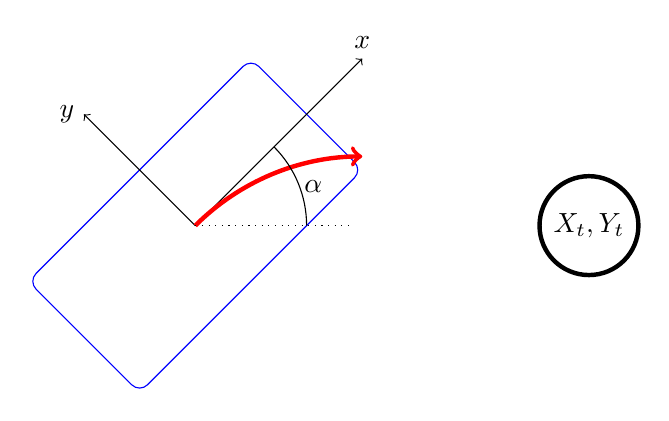
\begin{tikzpicture}
\begin{scope}[rotate=45]
\draw[rounded corners,blue] (-2,-1) rectangle (2,1);
\draw[->] (0,0)--(3,0) node[above] {$x$};
\draw[->] (0,0)--(0,2) node[left] {$y$};
\uncover<5->{
\draw[->,red,ultra thick] (0,0) arc (90:45:3);
}
\end{scope}
\draw[dotted](0,0)--(2,0);
\draw (1,1) arc (45:0:1.414);
\node at (1.5,0.5) {$\alpha$};
\uncover<2->{
\node[draw,ultra thick,circle] at (5,0) {$X_t,Y_t$};
}
\end{tikzpicture}
\uncover<3->{$$
(X_t,Y_t)\rightarrow(X_r,Y_r)
$$}
\uncover<4->{$$
\Delta\alpha=\arctan Y_r/X_r
$$}
\end{frame}

\begin{frame}\frametitle{Вероятностный подход}
\uncover<+->{$$
F_A(x)=P\{ A\le x \}
$$}
\uncover<+->{$$
F_A(x)=\int_{-\infty}^{x} f_A(x) dx
$$}
\uncover<+->{$$
P \{ A=x \} =0
$$}
\uncover<+->{
\begin{tikzpicture}[x=2cm,y=2cm]
\draw[->,thick] (0,0.01) -- (4.5,0.01) node[below] {$d$};
\draw[->,thick] (0,0) -- (0,1.2) node[left] {$f_A$};
\draw[red,thick] plot file {Plots/2.txt};
\end{tikzpicture}
}
\end{frame}

\begin{frame}\frametitle{Вероятностный подход}
 
\citate{
... в этом курсе, нас интересуют исключительно вероятностные распределения по конечному числу событий, 
поэтому нетривиальные вопросы интегрируемости, измеримости и т.д. мы рассматривать не будем.

Мне кажется, что теория вероятностей -- очередной пример того, как математики немедленно переходят 
в бесконечномерные пространства, в первую очередь для того, чтобы решить проблему отсутствия подходящей проблемы для решения.
Я не осуждю это, но в компьютерных науках даже количество вариантов $2^n$ очень велико. А уж число вариантов $2^{\aleph_0}$ нам нужно, 
как лишняя дырка в голове.

}{Scott Aaronson}{Quantum computing since Democritus}

\end{frame}

\begin{frame}\frametitle{Вероятностный подход}

\uncover<+->{$$
\mathbb{D}=\{d_{-k},d_{-k+1},\ldots,d_0=0,d_1=\varepsilon,d_2=2\varepsilon,\ldots,d_k\gg 0\}
$$}
\uncover<+->{$$
x=d_i\ \Leftrightarrow\ x\in[d_i-\varepsilon/2,d_i+\varepsilon/2)
$$}
\uncover<+->{$$
P \{A=a\}=K_A \cdot f_A(a)
$$}
\uncover<+->{$$
K_A\ :\ \left[\sum_{a\in\mathbb{D}} P\{A=a \}\right]=1
$$}


\end{frame}

\begin{frame}

\uncover<+->{$$
h:\mathbb{R}\times\mathbb{R}\rightarrow\mathbb{R}
$$}
\uncover<+->{$$
C=h(A,B)
$$}
\uncover<+->{$$
P\{ C=c \}=\sum_{a,b\ :\ h(a,b)=c} P\{ A=a\ \cap\ B=b\}=
$$}
\uncover<+->{$$
=\sum_{a,b\ :\ h(a,b)=c} P\{ A=a \}P\{ B=b \}=
$$}
\uncover<+->{$$
= K_C\cdot \sum_{a,b\ :\ h(a,b)=c} f_A(a)f_B(b)
$$}

\end{frame}

\begin{frame}\frametitle{Точное вычисление нечетких операций}

\uncover<+->{$$
\mu_X(x)=\max\left[0,1-\left(\frac{x-\ceil{X}}{q}\right)^2\right]
$$
$$
\mu_Y(y)=\max\left[0,1-\left(\frac{x-\ceil{Y}}{q}\right)^2\right]
$$
$$
Z=\arctan Y/X
$$}
\uncover<+->{$$
\mu_Z(z)=\max_{x,y\ z=\arctan(y/x)}\mu_X(x)\mu_Y(y)
$$}
\uncover<+->{$$
z=\arctan(y/x)\Rightarrow y=x \tan z
$$}
\uncover<+->{$$
\mu_C(z)=\max_{x\in\mathbb{X}}\left(1-(px-q)^2\right)\left(1-(rx-s)^2\right)
$$}
\end{frame}

\begin{frame}\frametitle{Точное вычисление нечетких операций}
$$
\mu_C(z)=\max_{x\in\mathbb{X}}\left(1-(px-q)^2\right)\left(1-(rx-s)^2\right)
$$
\only<2>{
\includegraphics[width=\textwidth]{wolfram.png}}
\only<3>{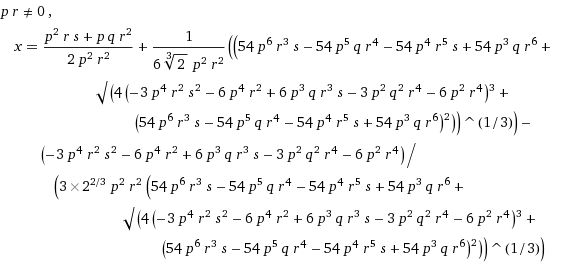
\includegraphics[width=\textwidth]{roots.png}}

\end{frame}

\section{Нечеткий вывод}

\begin{frame}
 \bio{Mamdani}{Ebrahim Mamdani}{Application of fuzzy algorithms for the control of a simple dynamic plant (1974)}
\end{frame}


\begin{frame}\frametitle{Нечеткий вывод}
\uncover<+->{\begin{center}
Если цель слева, надо повернуть налево.
\end{center}}
\uncover<+->{$$
\mu_L(y)=\left\{\begin{array}{l l}
                 0, & y<0 \\
                 y/M & y\ge 0 \\
                \end{array}\right.
$$}
\uncover<+->{$$
\mu_{TL}(\alpha)=1-(x-\pi/4)^2
$$}
\uncover<+->{$$
\mu_{\imp{L,TL}{G}}(y,\alpha)=\imp{}{G}\left[\mu_L(y),\mu_R(\alpha)\right]
$$}
\uncover<+->{$$
\imp{}{G}(a,b)=\min(1,b/a)
$$}
\uncover<+->{$$
\mu_{\imp{L,TL}{G}}(\alpha)=\max_{y\in\mathbb{R}}\mu_Y(y)\mu_{\imp{L,TL}{G}}(y,\alpha)=
$$}
\uncover<+->{$$
=\max_{y\in\mathbb{R}}\left[\mu_Y(y)\min(1,\mu_L(y)/\mu_TL(\alpha))\right]
$$}
\end{frame}

\begin{frame}\frametitle{Нечеткий вывод}
\begin{center}
Если цель слева, надо повернуть налево.
А если справа, то направо.
\end{center}

$$
\alpha=\left|\imp{L,TL}{G}(Y)\fcap \imp{R,TR}{G}(Y)\right|
$$
\end{frame}

\begin{frame}\frametitle{Нечеткий вывод}
\begin{center}
Если цель слева (L) и достаточно далеко (F), надо повернуть налево (TL).
\end{center}

\uncover<+->{$$
L(y)\wedge F(x)\rightarrow TL(\alpha)
$$}

\uncover<+->{$$
(y \fin L) \fwedge (x\fin F)\imp{}{G} (\alpha\fin TL)
$$}

\uncover<+->{$$
\imp{L\wedge F,TL}{G}=\imp{}{G}\left( \mu_L(y)\fwedge \mu_R(x), \mu_TL(\alpha)\right)
$$}

\uncover<+->{$$
\imp{L\wedge F,TL}{G}=\imp{}{G}\left( \mu_L(y)\mu_R(x), \mu_TL(\alpha)\right)
$$}


\end{frame}


\end{document}
